% To be compiled by XeLaTeX, preferably under TeX Live.
% LaTeX source for ``Yanqi Lake Lectures on Algebra'' Part III.
% Copyright 2019  李文威 (Wen-Wei Li).
% Permission is granted to copy, distribute and/or modify this
% document under the terms of the Creative Commons
% Attribution-NonCommercial 4.0 International (CC BY-NC 4.0)
% https://creativecommons.org/licenses/by-nc/4.0/

% To be included
\chapter{Some aspects of Koszul complexes}

This lecture is a faithful replay of the relevant sections of \cite{Bour80} and \cite{Bour98}; the main aim here is to complete the proof of Theorem \ref{prop:regular-vs-depth}. In what follows, we work with a chosen ring $R$. We impose no Noetherian or finiteness conditions here.

\section{Preparations in homological algebra}
For any $R$-module $L$, denote its \emph{exterior algebra}\index{exterios algebra} over $R$ by
\[ \bigwedge L := \bigoplus_{n \geq 0} \bigwedge^n L. \]
It is the quotient of the tensor algebra $T(L) = \bigoplus_{n \geq 0} (T^n(L) := L^{\otimes n})$ by the graded ideal generated by the pure tensors
\[ \cdots \otimes x \otimes x \otimes \cdots, \quad x \in L. \]
The multiplication operation in $\bigwedge L$ is written as $\wedge$. Note that $\bigwedge^0 L = T^0(L) = R$ by convention. The traditional notion of exterior algebras encountered in differential geometry is recovered when $\Q \subset R$.

Given $u \in \Hom_R(L, R)$, one can define the corresponding \emph{contractions} $i_u: \bigwedge^{n+1} L \to \bigwedge^n L$, given concretely as
\[ i_u (x_0 \wedge \cdots \wedge x_n) = \sum_{i=0}^n (-1)^i u(x_i) \cdot x_0 \wedge \cdots \widehat{x_i} \cdots \wedge x_n \]
where $\widehat{x_i}$ means $x_i$ is omitted. It is routine to check that $i_u$ satisfies $i_u \circ i_u = 0$, thereby giving rise to a chain complex.

\begin{definition}\label{def:Koszul-general}\index{Koszul complex}
	Let $L$ and $u$ be as above. Define the corresponding \emph{Koszul complex} as $K_\bullet(u) := (\bigwedge^\bullet L, i_u)$. For any $R$-module $M$, put
	\begin{align*}
		K_\bullet(u; M) & := M \dotimes{R} K_\bullet(u), \\
		K^\bullet(u; M) & := \Hom_A(K_\bullet(u), M)
	\end{align*}\index{$K^\bullet(u; M)$}
	which is naturally a chain (resp. cochain) complex in positive degrees; here one regards $M$ as a complex in degree zero. These definitions generalize to the case of any complex $M$, and are functorial in $M$.
\end{definition}

The reader might have encountered the following result in differential geometry.
\begin{proposition}[Homotopy formula]
	For any $x \in L$ and $\omega \in \bigwedge^n L$, we have
	\[ i_u (x \wedge \omega) + x \wedge (i_u(\omega)) = u(x) \omega. \]
\end{proposition}
\begin{proof}
	Consider $\omega = x_1 \wedge \cdots \wedge x_n$. Put $x_0 := x$. The left-hand side equals
	\[ \sum_{i=0}^n (-1)^i \cdot u(x_i) \cdots \wedge \widehat{x_i} \wedge \cdots  \]
	whereas the right-hand side equals
	\[ \sum_{i=1}^n (-1)^{i+1} \cdot u(x_i) x_0 \wedge \cdots \wedge \widehat{x_i} \wedge \cdots. \]
	The terms with a $\widehat{x_i}$ (non-existant --- hopefully this won't generate metaphysical issues) where $i > 0$ cancel out. We are left with $u(x_0) x_1 \wedge \cdots \wedge x_n = u(x) \omega$.
\end{proof}
Obviously, the same formula extends to all $\omega \in \bigwedge L$ by linearity.

\begin{proposition}\label{prop:Koszul-u-vanishing}
	Set $\mathfrak{q} := u(L)$, which is an ideal of $R$. Then $\mathfrak{q}$ annihilates each homology (resp. cohomology) of $K_\bullet(u; M)$ (resp. $K^\bullet(u; M)$). Again, this generalizes to general complexes $M$.
\end{proposition}
\begin{proof}
	Given $t \in \mathfrak{q}$, the homotopy formula implies that the endomorphism $\omega \mapsto t\omega$ of $K_\bullet(u)$ is homotopic to zero, hence so are the induced endomorphisms of $K_\bullet(u; M)$ and $K^\bullet(u; M)$ by standard homological algebra.
\end{proof}

\begin{proposition}\label{prop:Koszul-long-exact-sequence}
	Suppose $L$ is projective over $R$ and $0 \to M' \to M \to M'' \to 0$ is exact. Then there is a natural short exact sequence of complexes
	\[ 0 \to K^\bullet(u; M') \to K^\bullet(u; M) \to K^\bullet(u; M'') \to 0 \]
	which gives rise to a long exact sequence of cohomologies of the Koszul complexes in question.
\end{proposition}
\begin{proof}
	Standard. It suffices to note that $L$ is projective implies each graded piece $\bigwedge^n L$ of $\bigwedge L$ is projective as well.
\end{proof}

\begin{exercise}
	Justify the assertion above concerning the projectivity of $\bigwedge^n L$. Hint: suppose $L$ is a direct summand of a free module $F$, show that $\bigwedge^n L$ is a direct summand of $\bigwedge^n F$ and $\bigwedge^n F$ is free.
\end{exercise}

Similar properties hold for the homological version when $L$ is flat over $R$. One needs the property that $\bigwedge^n L$ is flat if $L$ is.
\begin{exercise}
	Prove the assertion above concerning flatness of $\bigwedge^n L$. Consult the proof in \cite[p.15]{Bour80} if necessary.
\end{exercise}

\section{Auxiliary results on depth}
We fix an ideal $I \subset R$.
\begin{proposition}\label{prop:depth-prod}
	For every family $\{M_\beta\}_{\beta \in \mathcal{B}}$ of $R$-modules, we have
	\[ \mathrm{depth}_I\left(\prod_\beta M_\beta \right) = \inf_\beta \mathrm{depth}_I(M_\beta). \]
\end{proposition}
\begin{proof}
	This follows from $\Ext^n_R(R/I, \prod_i M_i) = \prod_{i \in I} \Ext^n_R(R/I, M_i)$, as is easily seen by taking a projective resolution of $R/I$ and using the fact the $\Hom_R$ preserves direct products in the second variable.
\end{proof}

\begin{remark}
	By stipulation, the empty product is $0$, the zero object of the category $R\dcate{Mod}$. In parallel we define $\inf\emptyset := \infty$, so that Proposition \ref{prop:depth-prod} remains true in this case, since the zero module has infinite depth.
\end{remark}

\begin{proposition}
	Suppose $N$ is an $R$-module annihilated by some $I^m$, where $m \geq 1$. Then $\Ext^i_R(N,M)=0$ whenever $i < \mathrm{depth}_I(M)$.
\end{proposition}
\begin{proof}
	To show $\Ext^i_R(N,M)=0$ for $i < \text{depth}_I(M)$, we begin with the case $m=1$. This case follows by a dimension-shifting argument based on the short exact sequence
	\[ 0 \to K \to (R/I)^{\oplus I} \to M \to 0, \]
	together with induction on $i$ (note that $\Ext^{<0}_R(N,M)=0$ for trivial reasons). The case of general $m$ follows by a standard \emph{dévissage} using
	\[ 0 \to JN \to N \to N/JN \to 0 \]
	and the associated long exact sequence.
\end{proof}

\begin{lemma}\label{prop:depth-power}
	Suppose $J$ is an ideal satisfying $J \supset I^m$ for some $m \geq 1$. Then $\mathrm{depth}_I(M) \leq \mathrm{depth}_J(M)$.
\end{lemma}
\begin{proof}
	From the previous Proposition, we have $\Ext^i_R(R/J, M) = 0$ for $i < \text{depth}_I(M)$ since $I^m$ annihilates $R/J$. The assertion follows upon recalling the definition of depth.
\end{proof}

The following technical results will be invoked in the proof of Theorem \ref{prop:Koszul-depth}.
\begin{proposition}\label{prop:depth-vanishing-aux}
	Let $C^\bullet$ be a cochain complex of $R$-modules such that $n \ll 0 \implies C^n = 0$. Let $h \in \Z$  such that for all integers $n \leq k \leq h$, the depth of $C^n$ with respect to $J_k := \mathrm{ann}(H^k(C^\bullet))$ is $> k-n$, then
	\[ H^{\leq h}(C^\bullet)=0. \]
\end{proposition}
In what follows, we write $H^n = H^n(C^\bullet) = Z^n/B^n$ in the usual notation for homological algebra.
\begin{proof}
	Assume on the contrary that there exists $k \leq h$ with $H^{< k} = 0$ whereas $H^k \neq 0$. Write $J = J_k$. As $J$ annihilates the nonzero $R$-module $H^k$, the criterion of depth-zero modules (Proposition \ref{prop:depth-zero}) implies that $\text{depth}_J(H^k) = 0$. By assumption $\text{depth}_J(C_k) > k-k = 0$, it follows that $\text{depth}_J(Z_k) > 0$ since $Z_k \subset C_k$, by applying the aforementioned criterion of depth-zero. From the short exact sequence
	\[ 0 \to B^k \to Z^k \to H^k \to 0 \]
	we deduce distinguished triangles in $D(R\dcate{Mod})$
	\begin{gather*}
		\mathcal{H}\text{om}(R/J, B^k) \to \mathcal{H}\text{om}(R/J, Z^k) \to \mathcal{H}\text{om}(R/J, H^k) \xrightarrow{+1}, \\
		\mathcal{H}\text{om}(R/J, H^k)[-1] \to \mathcal{H}\text{om}(R/J, B^k) \to \mathcal{H}\text{om}(R/J, Z^k) \xrightarrow{+1}.
	\end{gather*}
	As the leftmost and rightmost terms of the last line are in $D^{\geq 1}(R\dcate{Mod})$, we see
	\[ \text{depth}_J(B^k) \geq 1; \]
	moreover, the piece $\Ext_R^0(R/J, Z^k) \to \Ext_R^0(R/J, H^k) \to \Ext_R^1(R/J, B^k)$ from the long exact sequence shows that $\text{depth}_J(B^k) = 1$. Now for $n < k$ we have short exact sequences
	\[ 0 \to \underbracket{B^n}_{= Z^n} \to C^n \to B^{n+1} \to 0. \]
	Again, one infers from the distinguished triangle
	\[ \mathcal{H}\text{om}(R/J, B^{n+1})[-1] \to \mathcal{H}\text{om}(R/J, B^n) \to \mathcal{H}\text{om}(R/J, C^n) \xrightarrow{+1} , \]
	the assumption $\text{depth}_J(C^n) > k-n$ and descending induction on $n$ that $n < k \implies \text{depth}_J(B_n) = k-n+1$. This is impossible since $B_{\ll 0} = 0$ has infinite depth.
\end{proof}

\begin{corollary}\label{prop:depth-vanishing}
	Let $I \subset R$ be an ideal, $C^\bullet$ be a cochain complex with $n \ll 0 \implies C_n=0$, and $h \in \Z$. Suppose that $n \leq h$ implies $I \cdot H^n(C^\bullet) = 0$ and $\mathrm{depth}_I(C^n) > h-n$. Then $H^{\leq h}(C^\bullet) = 0$.
\end{corollary}
\begin{proof}
	For $k \leq h$ we have $J_k := \text{ann}(H^k(C^\bullet)) \supset I$. Hence Lemma \ref{prop:depth-power} entails that
	\[ n \leq k \leq h \implies \text{depth}_{J_k}(C^n) \geq \text{depth}_I(C^n) > h-n \geq k-n. \]
	Now apply Proposition \ref{prop:depth-vanishing-aux}.
\end{proof}

\section{Koszul complexes and depth}
The simplest Koszul complexes are defined as follows. Given $x \in R$, we form the cochain complex in degrees $\{0,1\}$
\[ K(x) := \left[ R \xrightarrow{x} R \right]. \]
More generally, for any $R$-module $M$, viewed as a complex concentrated in degree zero, and a family $\mathbf{x} = (x_\alpha)_{\alpha \in \mathcal{A}}$ of element of $R$, we define the associated \emph{Koszul complex}\index{Koszul complex} as
\[ K^\bullet(\mathbf{x}; M) := K^\bullet(u; M), \]
where we take $u: R^{\oplus \mathcal{A}} \to R$ corresponding to $\mathbf{x}$ in Definition \ref{def:Koszul-general}. Unfolding definitions, we have \index{$K^\bullet(\mathbf{x};M)$}
\[ K^h(\mathbf{x}; M) = \begin{cases}
	\Hom_R\left( \bigwedge^h (R^{\oplus \mathcal{A}}), M \right), & h \geq 0 \\
	0, & h < 0. 
\end{cases} \]
Therefore $K^h(\mathbf{x}; M)$ consists of families $m(\alpha_1, \ldots, \alpha_h) \in M$ that are alternating in the variables $\alpha_1, \ldots, \alpha_h \in \mathcal{A}$. The differential is
\begin{align*}
	\partial^h: K^h(\mathbf{x}; M) & \longrightarrow K^{h+1}(\mathbf{x}; M) \\
	m & \longmapsto \left[ (\alpha_0, \ldots, \alpha_h) \mapsto \sum_{j=0}^h (-1)^j x_{\alpha_j} \cdot m(\ldots, \widehat{\alpha_j}, \ldots) \right].
\end{align*}
We shall abbreviate the cohomologies of $K^\bullet(\mathbf{x}; M)$ as the \emph{Koszul cohomologies}.

When $\mathcal{A} = \{1, \ldots, n\}$ we revert to
\[ K^\bullet(x_1, \ldots, x_n; M) := M \otimes K(x_1) \otimes \cdots \otimes K(x_n) \]
with the well-known sign convention. Also note that $R^{\oplus \mathcal{A}}$ is projective, hence the Proposition \ref{prop:Koszul-long-exact-sequence} can always be applied to Koszul cohomologies.

Let $I$ denote the ideal generated by $\{x_\alpha: \alpha \in \mathcal{A} \}$. The reader is invited to verify that
\begin{itemize}
	\item $K^\bullet\left( \mathbf{x}, \prod_{\beta \in \mathcal{B}} M_\beta \right) = \prod_{\beta \in \mathcal{B}} K^\bullet(\mathbf{x}; M_\beta)$ for any family $\{M_\beta\}_{\beta \in \mathcal{B}}$ of $R$-modules, and same for their cohomologies;
	\item the $0$-th cohomology of $K^\bullet(\mathbf{x}; M)$ is $\Hom_R(R/I, M) = \{x \in M: Ix=0 \}$, the $I$-torsion part of $M$;
	\item if $|A| = n$, the $n$-th cohomology of $K^\bullet(\mathbf{x}; M)$ is $M/IM$.
\end{itemize}
These facts will cast in our later arguments.

\begin{lemma}\label{prop:Koszul-coho-ann}
	Each cohomology of $K^\bullet(\mathbf{x}; M)$ is annihilated by $I$.
\end{lemma}
\begin{proof}
	Apply Proposition \ref{prop:Koszul-u-vanishing} by observing that $\mathfrak{q} = I$ in our setting.
\end{proof}

\begin{theorem}\label{prop:Koszul-depth}\index{depth}
	Let $M$ be an $R$-module and $\mathbf{x} = \{x_\alpha \}_{\alpha \in \mathcal{A}}$ be a family of elements of $R$, which generate an ideal $I$ of $A$. Then $\mathrm{depth}_I(M)$ equals
	\[ \inf \left\{n \geq 0: H^n(K^\bullet(\mathbf{x}; M)) \neq 0 \right\} \in \Z_{\geq 0} \sqcup \{\infty \} . \]
	Consequently, if $I \subset R$ is an ideal generated by elements $x_1, \ldots, x_n$ and $IM \neq M$, then we have
	\[ \mathrm{depth}_I(M) \leq n. \]
\end{theorem}
\begin{proof}
	Let $d := \text{depth}_I(M)$. Since $K^h(\mathbf{x}; M)$ is a direct product of copies of $M$ (possibly the empty product $=0$), by Proposition \ref{prop:depth-prod} its depth equals either $d$ or $\infty$. Combining Lemma \ref{prop:Koszul-coho-ann} and Corollary \ref{prop:depth-vanishing} (with $h = d-1$), we see that $H^{< d}(K^\bullet(\mathbf{x}; M)) = 0$. It remains to show $H^d(K^\bullet(\mathbf{x}; M)) \neq 0$ provided that $d < \infty$, which we assume from now onwards.

	The case $d=0$ is clear since there exists $\mathfrak{p} \in \text{Ass}(M) \cap V(I)$, therefore $R/\mathfrak{p} \hookrightarrow M$ and $\exists x \in M$ with $\mathfrak{p} x \supset Ix = \{0\}$, whence $H^0(K^\bullet(\mathbf{x}; M)) \neq 0$. Now suppose $d \in \Z_{\geq 1}$ and assume $H^d(K^\bullet(\mathbf{x}; M)) = 0$. Take a free resolution $F_\bullet \to R/I \to 0$ and put $C^\bullet := \Hom_R(F_\bullet, M)$, so that
	\[ H^i(C^\bullet) \simeq \Ext^i_R(R/I, M), \quad i \geq 0. \]
	Hence for $i < d$ we have short exact sequences
	\[ 0 \to B^i \to C^i \to B^{i+1} \to 0 \]
	as usual; recall $B^i, Z^i \subset C^i$. Note that each $C^i$ is a direct product of copies of $M$, hence $H^{\leq d}(K^\bullet(\mathbf{x}; C^i)) = 0$. Indeed, $H^{< d}(K^\bullet(\mathbf{x}; M))=0$ has been settled in the first step, whilst $H^d(K^\bullet(\mathbf{x}; M))$ is the hypothesis to be refuted. It then follows from the long exact sequence for Koszul cohomologies (Proposition \ref{prop:Koszul-long-exact-sequence}) that
	\[ (s \leq d) \wedge (i < d) \implies H^s(K^\bullet(\mathbf{x}; B^{i+1})) \hookrightarrow H^{s+1}(K^\bullet(\mathbf{x}; B^i)). \]
	Suppose $i < d$. As $B^0 = 0$, an iteration yields
	\[ H^{d-i}(K^\bullet(\mathbf{x}; B^{i+1})) \hookrightarrow \cdots \hookrightarrow H^{d+1}(K^\bullet(\mathbf{x}; B^0)) = 0. \]
	In particular, $i=d-1$ gives rise to $H^1(K^\bullet(\mathbf{x}; B^d)) = 0$. Hence the short exact sequence $0 \to B^d \to Z^d \to H^d \to 0$ (for $C^\bullet$) together with Proposition \ref{prop:Koszul-long-exact-sequence} give rise to
	\[ H^0(K^\bullet(\mathbf{x}; Z^d)) \twoheadrightarrow H^0(K^\bullet(\mathbf{x}; H^d)). \]
	As $H^d := H^d(C^\bullet) \simeq \Ext^d_R(R/I, M)$ is nonzero and annihilated by $I$, the right-hand side is nonzero. Hence $H^0(K^\bullet(\mathbf{x}; Z^d)) \neq 0$ and then $H^0(K^\bullet(\mathbf{x}; C^d)) \neq 0$, as the zeroth Koszul cohomology is nothing but the $I$-torsion part.
	
	Finally, recall that $C^d \neq \{0\}$ is a direct product of copies of $M$, consequently
	\[ H^0(K^\bullet(\mathbf{x}; M)) \neq 0. \]
	However, this contradicts the earlier result that $H^{<d}(K^\bullet(\mathbf{x}; M))=0$ since $d \geq 1$.
\end{proof}

This yields an alternative characterization of depth. It also completes the proof of Theorem \ref{prop:regular-vs-depth} as promised in the previous lecture.

% Finalizing...
\vfill
\begin{figure}[h]
	\centering 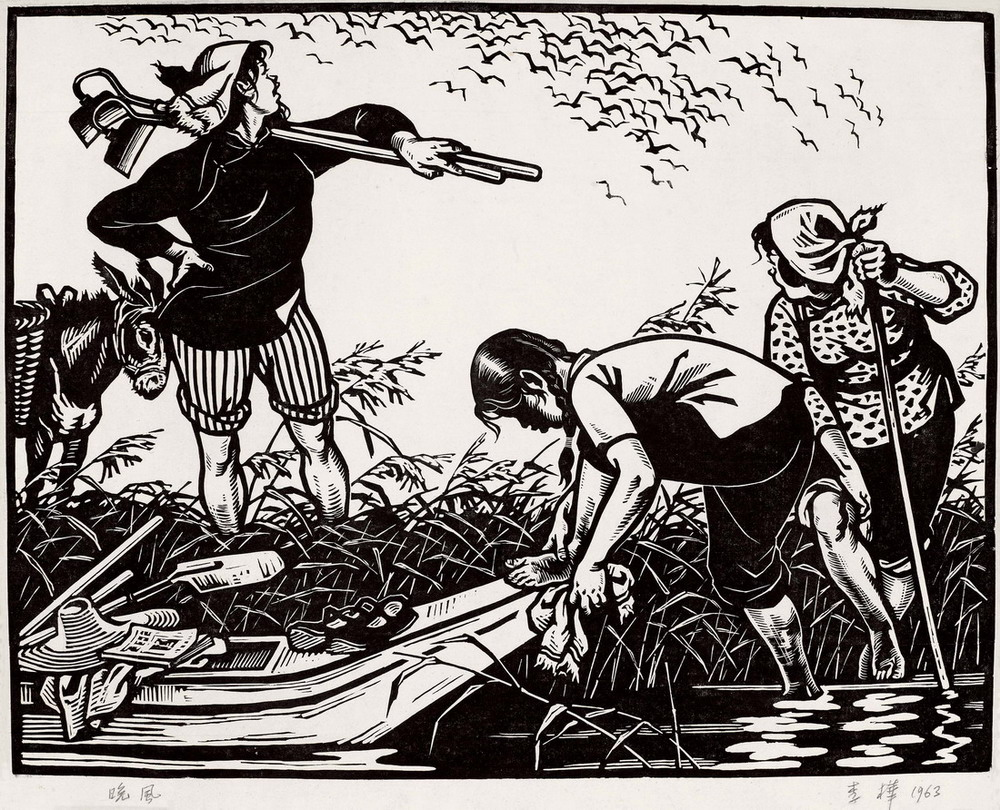
\includegraphics[height=200pt]{WanFeng.jpg} \\ \vspace{1em}
	\begin{minipage}{0.7\textwidth}\begin{center}
			\small \fontspec{Noto Serif CJK SC} 《晚风》, 李桦, 木刻版画, 1963 年.
	\end{center}\end{minipage}
\end{figure}
\vfill